\section{Background}
\subsection{System Monitoring}
System monitoring data consists of various system activities in the form of events along with time~~\cite{backtracking, backtracking2, taser,wormlog}. Each event can naturally be described as a system entity (subject) does some operation on another system entity (object). For example, a process reads a file or a process accesses a network connection. An APT attack needs multiple step to succeed , such as target discovery and data exfiltration, as illustrated in the cyber kill chain~\cite{killchain}. Therefore, multiple attack footprints might be left as "dots", which can be captured precisely by system monitoring. System monitoring data for Windows and Linux can be collected via ETW event tracing~\cite{etw} and Linux Audit Framework~\cite{auditd}. The audit framework used in this project is a popular and opensource audit application: Sysdig.
\begin{figure}
	\centering
	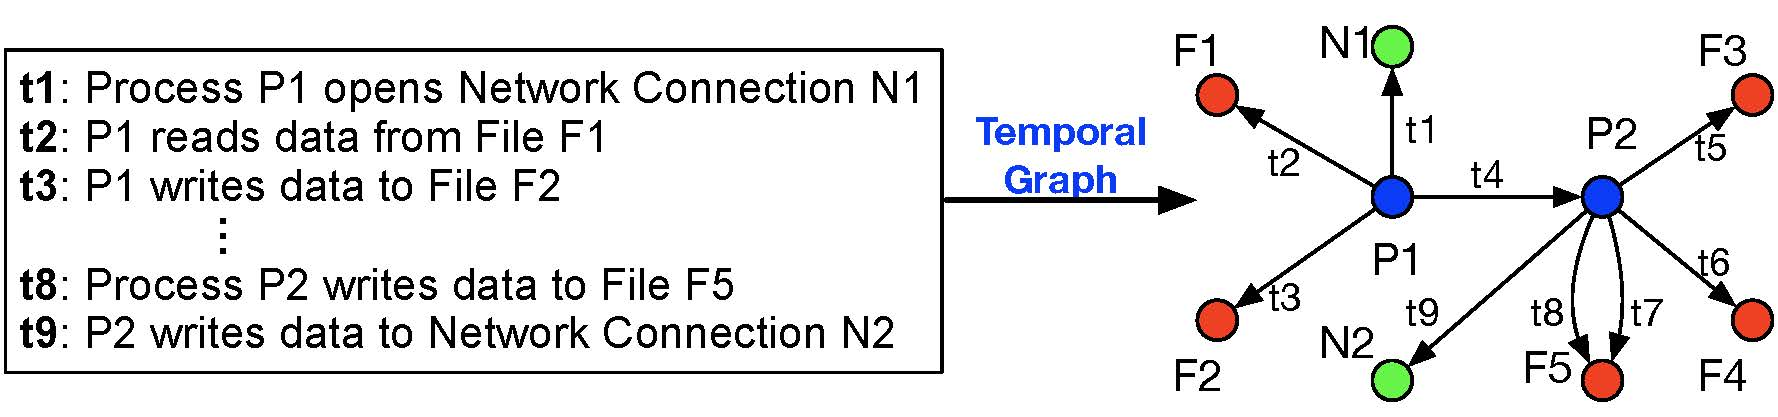
\includegraphics[width=0.48\textwidth]{temporal-graph.jpg}
	\caption{System monotoring Data}
	\label{fig:temporalGraph}
\end{figure}
\subsection{Sysdig}
Sysdig is a popular system and container monitoring tool. It improves the system and container visibility, combined with Kubernetes, Docker and Mesos integration, better record enterprises's services. It gives system manager an easy access to the actual behavior of the system and container. Far too often, system-level monitoring still involves logging into a machine with SSH and using plethora of dated tools with very inconsistent interfaces. Sysdig instruments physical and virtual machine at the operating system level by installing into the Linux kernel and capturing system calls and other system events.
\subsection{Output data description}
\begin{figure}[h]
	\centering
	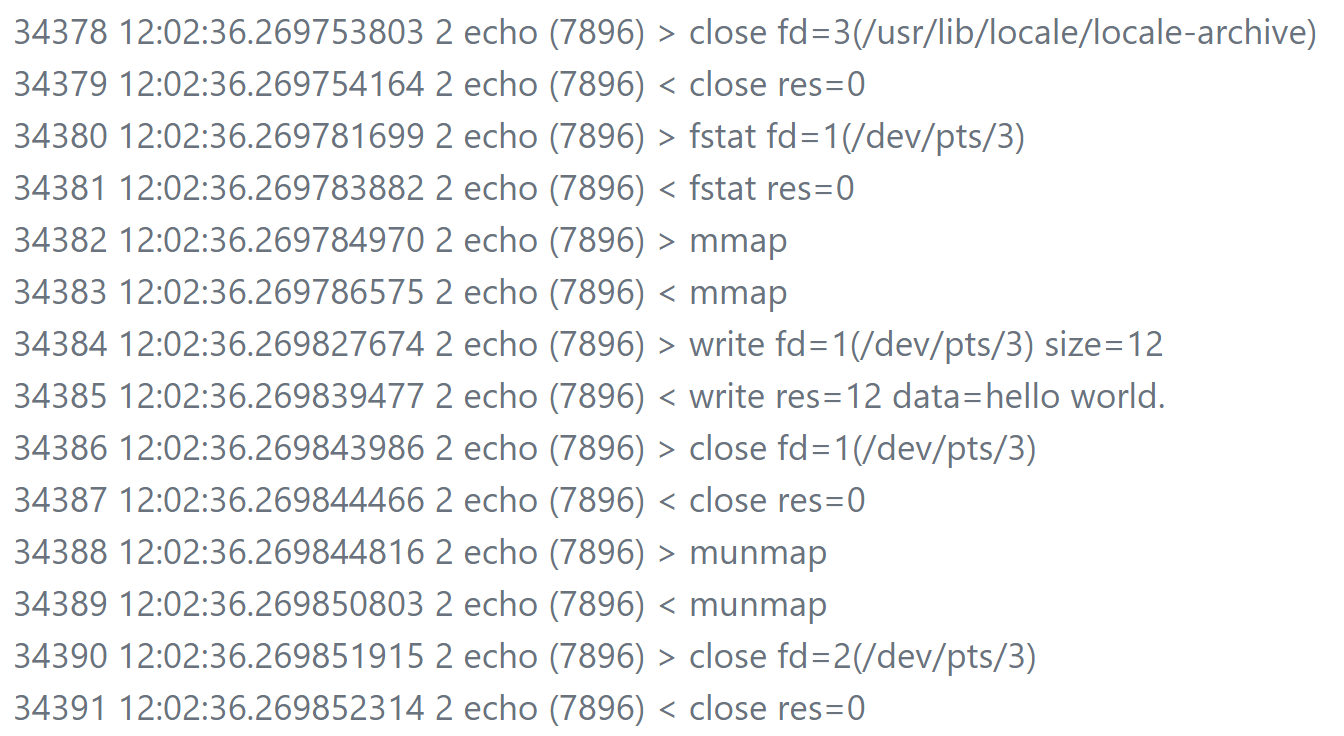
\includegraphics[scale=0.5]{fig1}
	\caption{Raw Data Output}
\end{figure}
The raw output data already includes many useful information, however it is still not enough to build the dependency graph of all the system behaviors. According to the Sysdig user guide, the output data format is defined as: 
\vspace{0.2em}

\noindent{\texttt{\%evt.num \%evt.rawtime.s.\%evt.rawtime.ns \%evt.cpu \\ \%proc.name (\%proc.pid) \%evt.dir \%evt.type cwd=\%proc.cwd \%evt.args latency=\%evt.latency}}

where:
\begin{itemize}[noitemsep]
	\item evt.num is the incremental event number.
	\item evt.rawtime.s is second part of the event timestamp.
	\item evt.rartime.na is nanosecond part of the event timestamp.
	\item evt.cpu is the CPU number where the event was captured
	\item proc.name is the name of the process that generated the event.
	\item proc.pid is the process id that generated the event
	\item evt.dir is the event direction, > for enter events < for exit events.
	\item evt.type is the name of system event e.g. `open' or `read'.
	\item proc.cwd is the current working directory of the event.
	\item evt.args is all the event agruments, aggregated into a single string.
	\item evt.latency is the delta between an exit event and the correspondent enter event in nanoseconds.
\end{itemize}
\begin{figure}
	\centering
	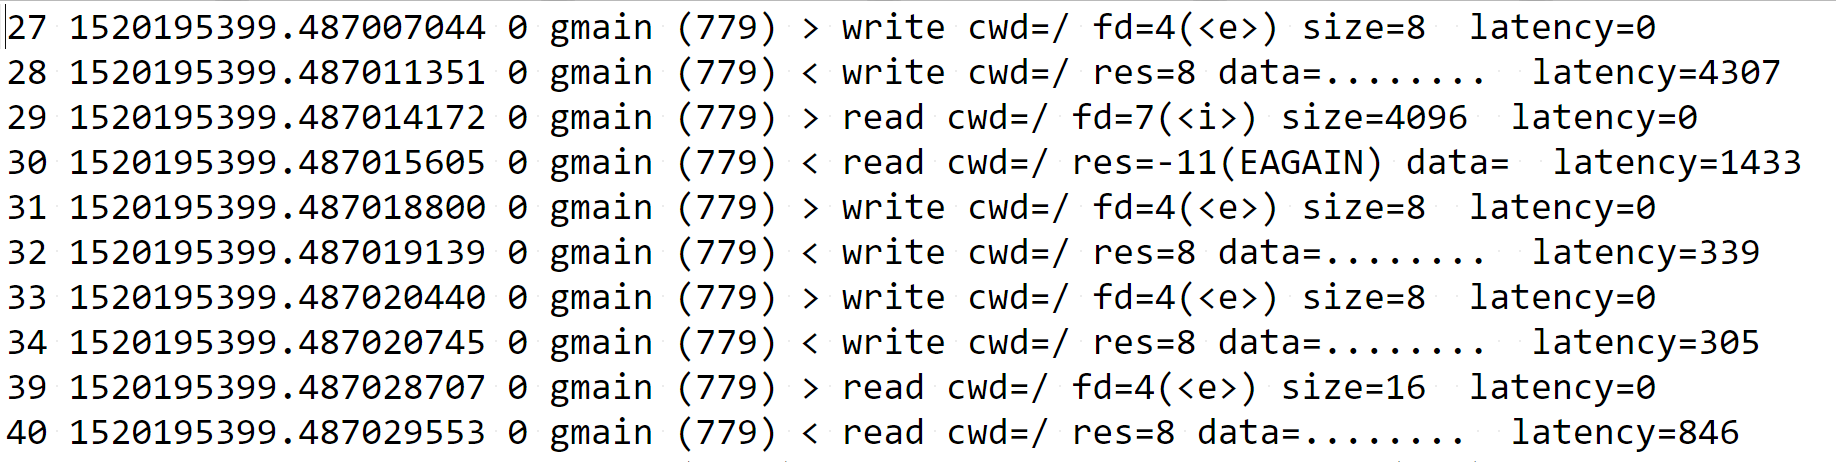
\includegraphics[scale=0.4]{fig2}
	\caption{Self-defined Data format}
\end{figure}
Currently, the information we try to gather includes events start time ,exit time, the id and name of the process that generated the event, the event arguments and duration. Based on the observation, the output data also includes many \textit{switch} events, which is generated by the CPU task scheduling algorithm. This information is too detail and unnecessary for the dependency graph analysis. The goal of system monitoring is to record the legal user's or unknown attacker's operation. Therefore, this  kind event can be safely neglected. In this project, there are three type system events need to be processed. The first type is about how a process is created. The relevant events are clone and fork in Linux system. The second type is file operations. The relevant event about this type are read, write and writev. The third type event is about network communication. The relevant system events are sendto. Through the filter provided by Sisdig, we can only gather the interested events.
%\subsection{Log Parser}
%After gathering the data, we need build the dependency graph based on the log file. There are three type vertexes representing three kind system entities: process, file and network communication.
%The identifier for process is its name and id.  For file, it is identified by its absolute file path, for network communication, it is distinguished by the communication two sides' ip and port number. We use three kind shape to represent these three system entities. According to the entities included in the system event, the parser need to process five kinds edge : process to process, process to file, file to process, network to process, process to network. The type of edge is decided by the event arguments. The output of Sysdig will use \textit{fd} as its identifier or key word. In the value part, it will use different characters to represent different objects.For example, it use \textit{f} to represent file, \textit{6} to represent IPV6 sockets,\textit{4} to represent IPV4 sockets. This kind information is necessary, without this, it is hard to know the start or end of information flow is a file or an ip address.  Through this way, the parser can know the kind of entities generating this event. For process to process event, we can directly know objects generating this event is two processes, because its event type is unique : fork or clone. In the conclusion, the parser will establish the dependency relationship between two system entities. This dependency relationship is specified by three parts: a source object, a sink object and a time interval$(t_s(e), t_e(e))$
\subsection{Dependency Anlysis}
Dependency analysis~~\cite{backtracking,backtrackingfile,backtracking2} plays an important role in security applications,
such as finding the entry points of attacks (\emph{causal analysis})
and investigating ramification of attacks (\emph{impact analysis}).
Given events $evt_1$ and $evt_2$, to construct a backward (forward) dependency $evt_1\xrightarrow{backward} evt_2$ ($evt_1\xrightarrow{forward} evt_2$), $evt_1$ must occur after (before) $evt_2$.

Backward dependency analysis can be used to analyze the \emph{causality} of an anomalous event,
such as the creation of an unknown executable in a system.
%Nowadays, executables in a computer are frequently updated, and thus not all malicious ones may be captured by anti-virus software. 
%To know whether an executable is safe to run, it is important to know whether it comes from trusted sources, such as Windows updates or official updaters like the Chrome updater.
Backward dependency analysis finds the origins of the executables by searching the events backward in time: 
(1) start the investigation of the processes that create the executables;
(2) from the processes, trace back to see which executables the processes executed;
(3) if the executables are from a trusted source, then we can stop the search; 
otherwise, the tracking continues until it finds the origin (such as installer files or downloaders).
As another example, forward dependency analysis helps users understand the ramification of malware.
Assume that we identified a malicious script in the web server. 
To understand how it infects a victim machine, we can start the investigation of the process that executed or read from the script,
and trace whether they propagate the malicious scripts across hosts
In this project, the goal of this step is to reconstruct the time line in an attack.
However, modern operation system is very complex, even through the user does not do any specific operation, it still has many service process running at the backend. That will generate many log records in the audit tool's output. In other words, these events will be represented as many edges and vertexes that we don't need. So we need to run backtrack~\cite{backtracking, backtracking2} from at least one \textit{detection point}~\cite{lamport1978time}, such as a modified, extra, or deleted file, or a suspicious or missing process. There are two standards to decide which system entity or operation is relevant to \textit{detection point} or not. The first one is whether there is a path existing between two vertexes or not. That means the source entity can use several operations to affect the state of the object entity. The second one is that the time intervals can be used to reduce false dependencies. For example, a process that reads a file at time 10 does not depend on writes to the file that that occur after time 10. Figure ~\ref{fig:simpleBack} record the key system entities of a file operation event: script $($writeFile.py$)$ use \textit{python} reads data from \textit{source.txt} and write these data to \textit{target.txt}.
\begin{figure}[!htb]
	\centering
	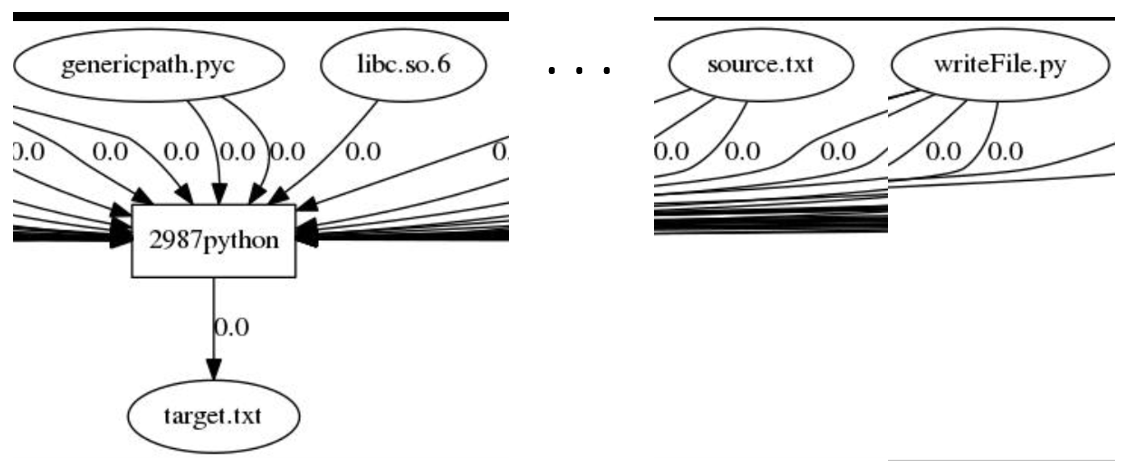
\includegraphics[width=0.5\textwidth]{simpleBack.png}
	\caption{Key System Entities Of Backtracking Result}
	\label{fig:simpleBack}
\end{figure}
%\begin{figure}[!htbp]
%	\centering
%	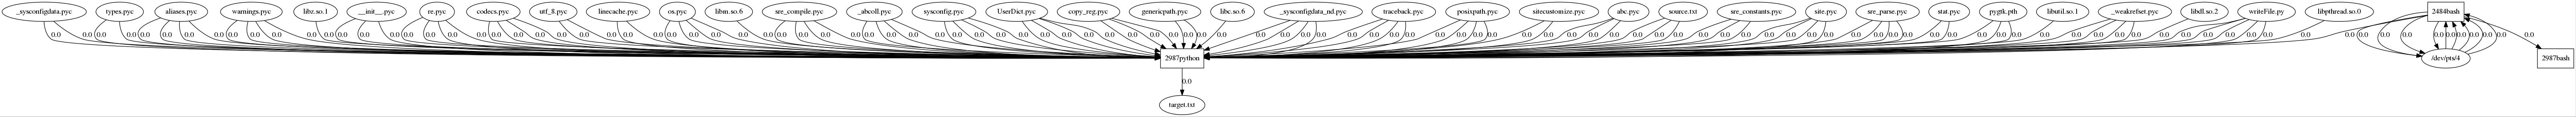
\includegraphics[width=1.3\textwidth,angle=90]{fileBack.jpg}
%	\caption{Backtracking of File operation}
%	\label{fig:backtrack}
%\end{figure}
\subsection{Causality Preserve Reduction}
\begin{figure}[!htb]
	\centering
	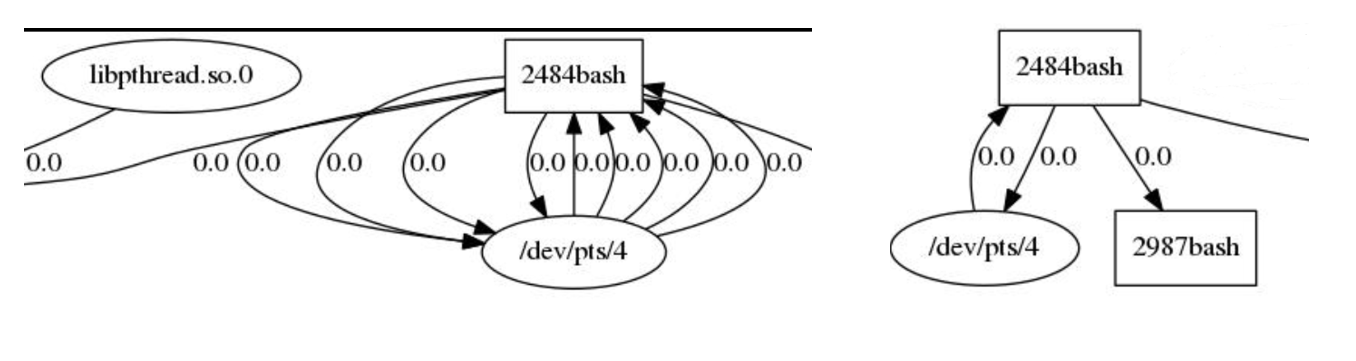
\includegraphics[width=0.5\textwidth]{simpleCPR.png}
	\caption{Causality Preserve Reduction Result}
	\label{fig:simpleCPR}
\end{figure}
From the graph processed by the Backtrack, it is not hard to notice that there are always multiple edges between the same pair of vertexes. This is because the number of operations is not equal to the log record number. For example, If one user try to read a file, the system will not read all data from disk at one time, it will read it hundreds or thousands times. In other words, many edges are corresponding to the same event. In a real-world scenario, an average desktop computer produces more than 1 million events per day, while a server could yield 10 to 100 times the volume. 
%Each day, a rather small system of 100 computers generated more than 200 million events, which requires mid- to high-end server to process and produces databases over 200GB. 
Reducing the data volume is key to solving the scalability problem. The difference between left part of Figure~\ref{fig:simpleCPR} and and right part of Figure~\ref{fig:simpleCPR} show the result of Causality Preserve Reduction$($CPR$)$. It is obvious that many edges connecting  process $2484bash$ and $/dev/pts/4$ is mergered by CPR.
%\begin{figure}[!htbp]
%	\centering
%	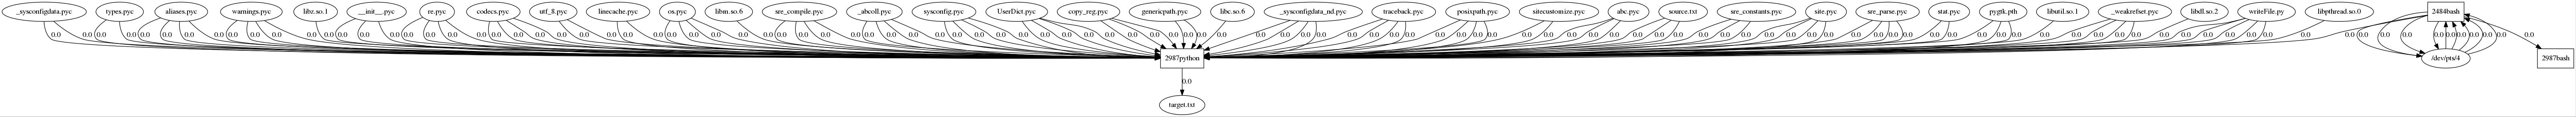
\includegraphics[width=1.3\textwidth,angle=90]{fileBack.jpg}
%	\caption{Backtracking of File operation}
%	\label{fig:CPR}
%\end{figure}
%\begin{figure*}[!hp]
%	\centering
%	\subfloat[Backtracking]{
%		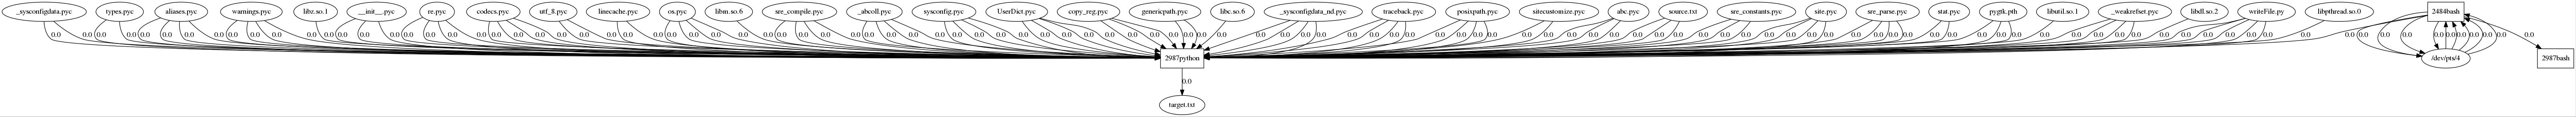
\includegraphics[align=c,width=1.3\textwidth, angle=90]{fileBack.jpg}}
%	\vfill
%	\subfloat[Causality Preserve Reduction]{
%		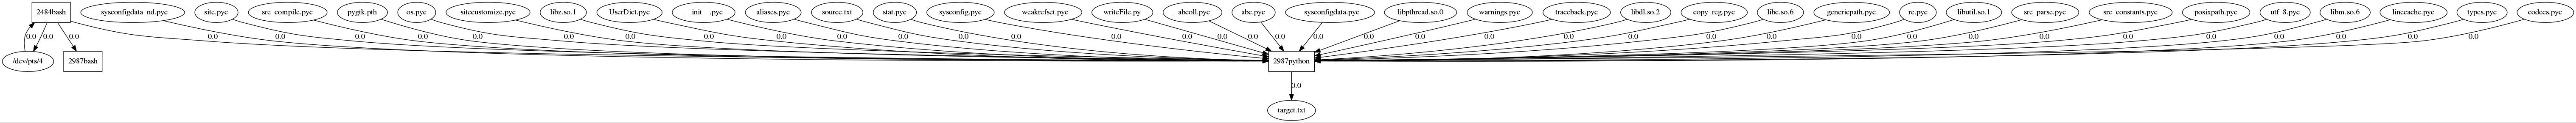
\includegraphics[align=c, width=1.3\textwidth,angle=90]{fileCPR.jpg}}
%\end{figure*}


%\begin{figure}[!htp]
%	\centering
%	\begin{minipage}{0.25\textwidth}
%		\centering
%		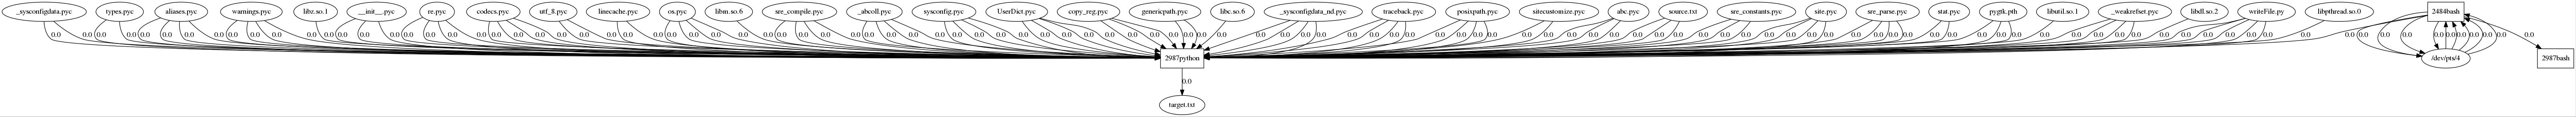
\includegraphics[align=c,width=\textheight, angle=90]{fileBack.jpg}
%		\caption{Backtracking}
%	\end{minipage}
%	\begin{minipage}{0.25\textwidth}
%				\centering
%				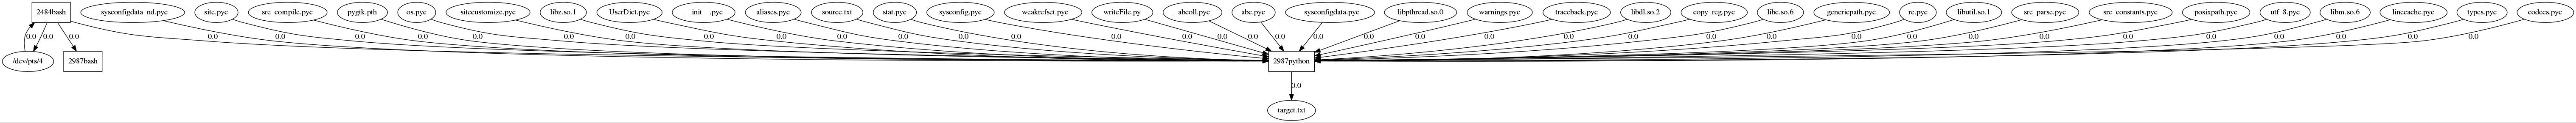
\includegraphics[align=c,width=\textheight, angle=90]{fileCPR.jpg}
%				\caption{CPR}
%	\end{minipage}
%\end{figure}

%While data reduction is a well-studies topic, the most commonly used techniques, spatial and temporal sampling, are not applicable to dependency analysis based on system event traces. Because sampling techniques do not have the inherit concept of causal relations, they are prone to introducing random causal errors. 


\begin{figure*}[!htp]
	\centering
	
	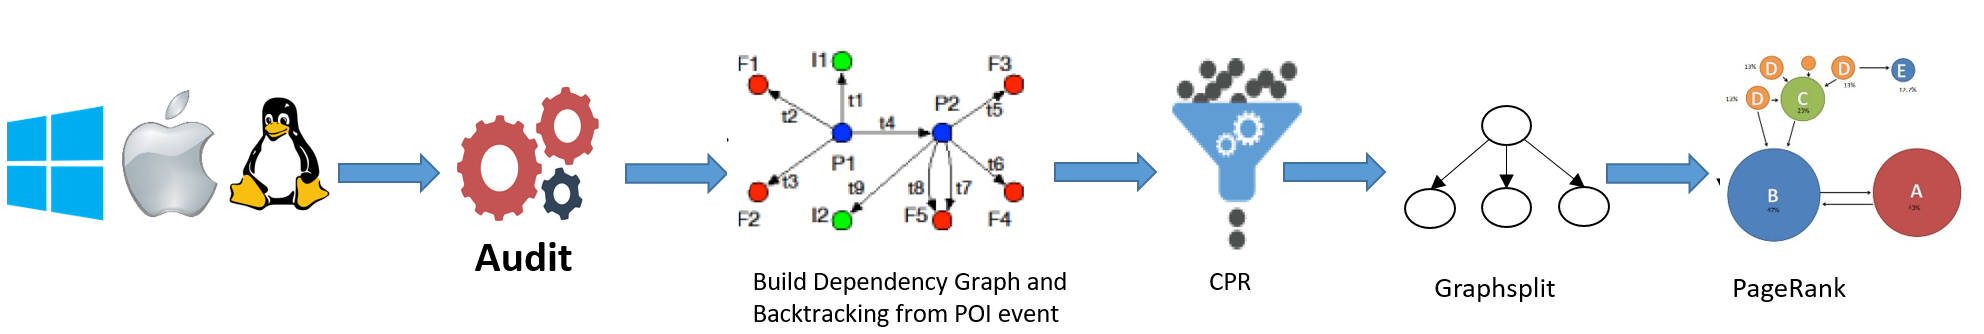
\includegraphics[width=\textwidth]{figflow2.png}
	\caption{Overview of automatic dependency analysis}
	\label{fig:steps}
\end{figure*}


\subsubsection{Design}
In this section,  we first present a formal definition of important terms and concepts used in our design.
First, two events have \textit{causality dependency} with each other if an event has information flow that affect the other event.\\
DEFINITION 1: \textbf{Causality Dependency} \\
\indent For two event edges $e_1 = \mathit{(u_1, v_1)} $ and $e_2 = \mathit{(u_2, v_2)} $ , they have causality dependency, if
\begin{itemize}[noitemsep]
	\item $v_1 = u_2 $
	\item $te\mathit{(e_1)} < te\mathit{(e_2)}$
\end{itemize}
if $e_1$ has information flow to $e_2$ and $e_2$  has information flow to $e_3$, then $e_1$ and $e_3$ have causality dependency.
Our primary reduction scheme aims at preserving causality dependency while performing the data reduction. For example, assuming there are multiple edges between the vertex $u$ and $v$, we need to check whether the merge of edges will break the backward trackability and forward trackability~~\cite{xu2016high}.We can merge the edges, if that merge will not loss the information about causality dependency.

%\subsection{Graph Split}
% PageRank~~\cite{pagerank} considers the World Wide Web as a set of linked nodes and ranks them based on their importance. The insight of PageRank is that a node linked by important nodes should be more important than the ones linked by uninfluenced nodes. That is, a web page's "reputation" is impacted by all the other web pages pointing to it. PageRank uses a transition matrix to represent the weights of edges from node \textit{j} to node \textit{i}. However,although Causality Preserve Reduction can merge many edges, there still may have multiple edges existing the same pair of nodes, because we don't want that the dependency relationship is lost during Causality Preserve Reduction. Therefore, we borrow the idea of static single assignment from(SSA)~~\cite{nielson2004principles}, splitting source node  into multiple nodes, where each of the split node has only one outgoing edge pointing to target node. We need duplicate all the edges originally pointing to source to each of the split node from node j.By replacing source node with the split nodes, we can then use PageRank to compute system entities' reputation.\\
% The basic idea for GraphSplit is that for every vertex$(V)$ of the dependency graph, we need to check its incoming edges. If several incoming edges share the same source, we declare a \textit{vertexPair} contains object $V$, source $S$ and a list of edges that connect these two vertexes. We maintain a queue for all $vertexPairs$. We also maintain a set of vertex has alread been  split.If we find the current $vertexPair.S$ or $vertexPair.V$ is split, then we just skip it in current round. We will split it in the next round. Here is the relvant function of GraphSplit.\clearpage
% \begin{algorithm}
%	\caption{GraphSplit}
%	\KwIn{A dependency Graph}
%	\SetKwFunction{FindPair}{FindPair}
%	\SetKwFunction{UpdateGraph}{UpdateGraph}
%	\SetKwFunction{RecoverTimeLogic}{RecoverTimeLogic}
%	\textbf{function}: GraphSplit$(\textit(G))$\\
%	$Queue$ $\leftarrow$ \FindPair{$G$}\;
%	\While{Queue is not Empty}{
%		$V$ $\leftarrow$ $Queue.poll()$\;
%		$S \leftarrow V.source$\;
%		$T \leftarrow V.target$\;
%		\If{Set contains S $or$ Set contains T}{continue}
%		$list1 \leftarrow$ list of outgoing edges of $S$ whose object is not $T$\;
%		$list2 \leftarrow$ V.list\;
%		\UpdateGraph($G$,$list1$,$list2$)\;
%		add $S$ to Set\;
%		$Queue \leftarrow$ \FindPair($G$)\;
%		}
%	\RecoverTimeLogic{$Set$}\;	
%\end{algorithm}
%\begin{algorithm}
%	\caption{FindPair}
%	\KwIn{A dependency Graph(G)}
%	\KwResult{A queue containing the vertex pair need to be splited}
%	\textbf{function}: FindPair$\textit(G)$\\
%	$V \leftarrow G.vertexSet$\;
%	\For{$v \in V$}{
%		$E \leftarrow$ incoming edges of $v$\;
%		\If{$\exists e \in E$ sharing the same source}{
%			$vertexPair.source \leftarrow e.source$\;
%			$vertextPair.object \leftarrow v$\;
%			$vertexPair.object.list$ add $e$\; 
%			$Queue$ add $vertexPair$\;}
%		}
%	\Return{Queue}
%\end{algorithm}
%\begin{algorithm}
%	\caption{RecoverTimeLogic}
%	\KwIn{A set of splited vertex}
%	\textbf{function}: RecoverTimeLogic$\textit(Set)$\\
%	$V \leftarrow G.vertexSet()$\;
%	\For{$v \in V$}{
%		\If{$v$ is the splitting node belongs to $Set$}{
%			$endtime \leftarrow$ the biggest endtime of outgoing edges of $v$\;
%			\For{$e \in$ incoming edges of v}{
%				\If{$e.start > endtime$}{remove this edge\;
%				}
%			}
%		}
%	} 	
%\end{algorithm}
%\begin{algorithm}
%	\caption{UpdateGraph}
%	\KwIn{A dependency Graph and.\\
%		 list1 is a list of outgoning edges of the source except edges whose object is V. \\
%		 list2 is a list containing edges between S and V}
%	\textbf{function}: UndateGraph$\textit(G, list1, list2)$\\
%	$list \leftarrow$ empty list of vertex\;
%	\For{$ e \in list2$}{
%		$u \leftarrow split(S)$\;
%		$list$ add $u$\;
%		$G$ add $u$\;
%		$G$ add a new edge from $u$ to $V$\;
%		}
%	\For{$u \in list$}{
%		\For{$e \in list1$}{
%			$G$ add a new edge from $u$ to the object of $e$\;}
%	}
%	\For{$u \in list$}{
%		\For{$e \in$ in the incoming edges of $S$}{
%			$G$ add a new edge from the source of $e$ to $u$\;}
%	}
%	remove $S$, the incoming and outgoing edges of $S$ from the $G$\;	
%\end{algorithm}
%\begin{algorithm}
%	\caption{RecoverTimeLogic}
%	\KwIn{A set of splited vertex}
%	\textbf{function}: RecoverTimeLogic$\textit(Set)$\\
%	$V \leftarrow G.vertexSet()$\;
%	\For{$v \in V$}{
%		\If{$v$ is the splitting node belongs to $Set$}{
%			$endtime \leftarrow$ the biggest endtime of outgoing edges of $v$\;
%			\For{$e \in$ incoming edges of v}{
%				\If{$e.start > endtime$}{remove this edge\;
%			}
%		}
%	}
%} 	
%\end{algorithm}
%\begin{figure*}[htp] 
%	\centering
%	\subfloat[original graph]{%
%		\includegraphics[width=0.5\linewidth,height=5cm]{sampleBeforeSplit.jpg}%
%		\label{fig:a}%
%	}%
%	\hfill%
%	\subfloat[after splitting]{%
%		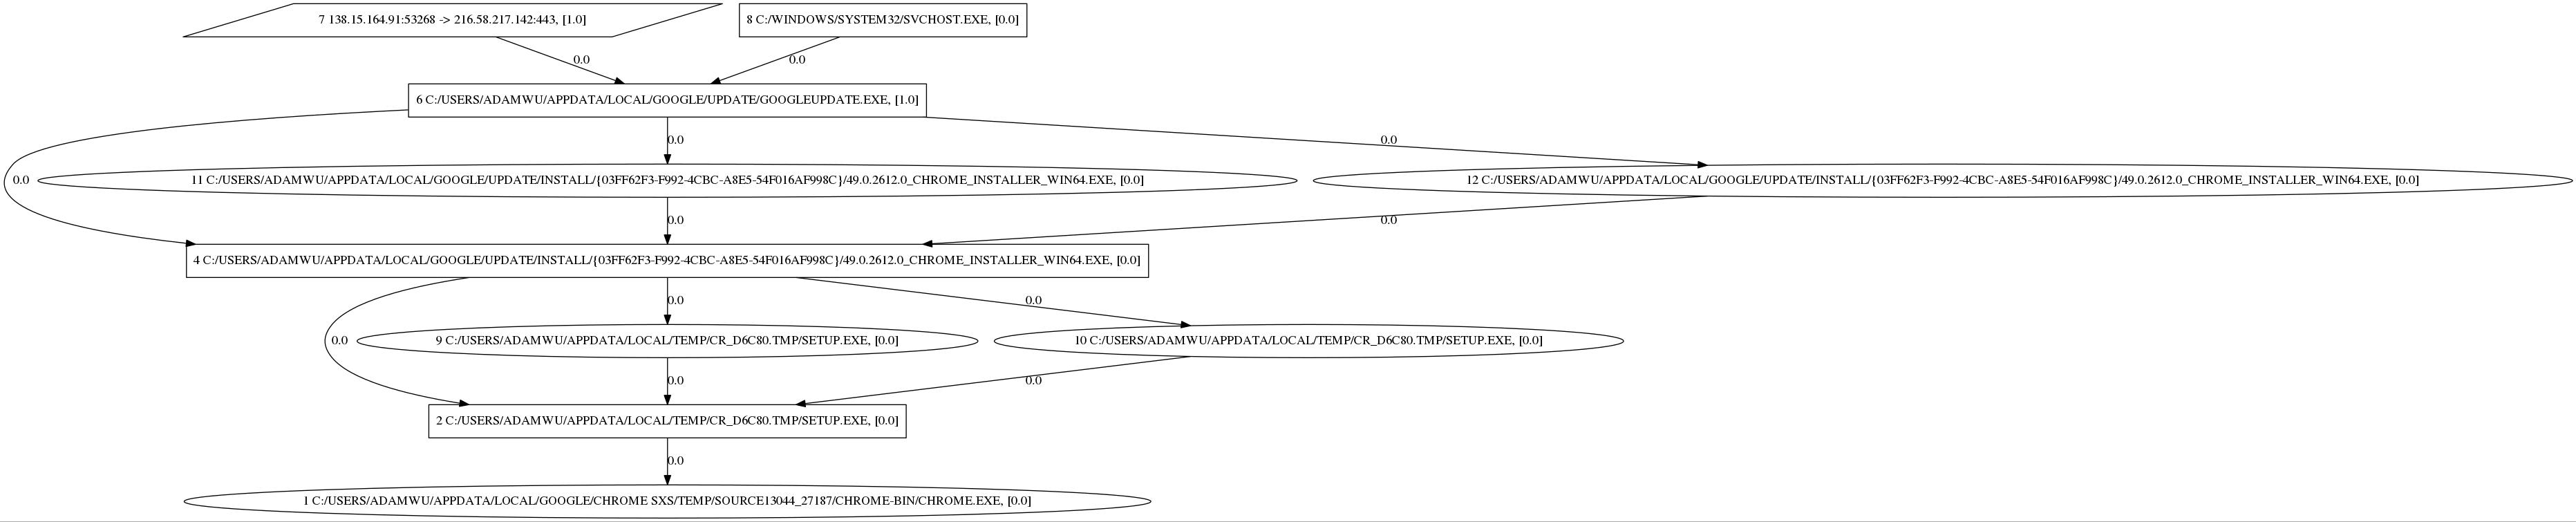
\includegraphics[width=0.5\linewidth,height=5cm]{splitTest.jpg}%
%		\label{fig:b}%
%	}%
%	\caption{The test sample of Graph Split}
%	\label{fig:sampleResult}
%\end{figure*}
